\chapter{The eScriptorium VRE for Manuscript Cultures}
\chaptermark{eScriptorium for Manuscript Cultures}
\thispagestyle{empty}
\vfill
This chapter has been accepted for publication in \fullcite{stokes2021escriptorium}
\newpage

\section{Introduction: What is eScriptorium}

The eScriptorium VRE is software being developed at the École Pratique des
Hautes Études, Université Paris Science et Lettres (EPHE – PSL), with the
immediate goal of developing a web interface to an engine for the automatic
transcription of written sources, both printed and handwritten, in principle in
any current or historical system of writing.\footnote{Further discussions and
papers on the eScriptorium project include
\cite{kiessling2019kraken,KiesslingEtAl2019eScrip, kiessling2019badam,
stokes2020escriptorium}. This work has received funding from the European
Union’s Horizon 2020 Research and Innovation program under Grant Agreement No.
871127 (RESILIENCE), and from the Initiatives de Recherches Interdisciplinaires
et Stratégiques of Université PSL (Scripta-PSL).} The software is intended to
be a core component in a larger VRE which provides the key steps in the normal
editorial chain. The assumption here is that the researcher has images of the
text, and wishes first to obtain a transcription of the text in these images,
then (most likely) add markup to the text and potentially also to the images in
order to encode the various editorial judgments that are a core part of any
edition, perhaps then also or instead to apply techniques such as Natural
Language Processing (NLP) or Named Entity Recognition (NER), and finally to
publish the text and image, along with accompanying data and metadata. To date,
the focus has been entirely on the first of these steps, that is, allowing the
manual, semi-automatic or automatic transcription of texts, and the user can
then export the results to be marked up, analyzed and/or published in other
frameworks.

The development of eScriptorium began as part of a larger project at PSL called
Scripta, which is studying the history and practice of writing in almost all
its forms across most of human history, and it has since been continued most
notably in the Resilience project, which is a European infrastructure project
looking to develop a long-term (35-year) research infrastructure for religious
studies. The range of languages and writing-systems being studied in the
Scripta project is enormous, covering the Ancient Near East (e.g. Ancient
Aramaic, Ptolemaic Egyptian, Ugaritic), Iran and Central Asia (including
Elamite, Sogdhian, Middle Iranian), India and South-East Asia (such as
Sanskrit, Classical Tamil, Old Javanese, Tai-Lue), and East Asia (Tibetan,
Classical Chinese, Old and medieval Japanese), as well as the Classical and
Medieval West (including Greek, Umbrian, and Old Slavonic), among others. The
scope of Resilience is in principle even bigger, as it should cover all
languages relevant to any aspect of religious studies in Europe for the next
thirty-five years. It has therefore been a crucial element of the project that
the software must avoid as far as possible all assumptions about the nature of
the writing and language that is in the system. The writing may be left to
right, right to left, top to bottom or even bottom to top; the support may be
paper, parchment, but also stone, palm leaf, clay, wood, or many others; it may
be written with a pen, painted with a brush, inscribed with a chisel; the
writing system may be alphabetic, logographic, hieroglyphic; and so on. This
variety means that almost all levels of the software are very much more complex
than they would be for a single type of script, as will be discussed below.

The eScriptorium VRE is designed to interface with the Kraken engine for
OCR/HTR.\footnote{Some writers distinguish Optical Character Recognition (OCR)
as the automatic transcription of printed text and Handwritten Text Recognition
(HTR) as that of handwritten text, whereas others reserve OCR for
character-based approaches to recognition and HTR for line-based. As a result,
the difference between OCR and HTR is often blurred in the current literature,
and so we use the two terms together as interchangeable unless clearly stated
otherwise.} This engine has been developed by Benjamin Kiessling, who is also
from EPHE-PSL and is part of the eScriptorium team. Written in Python, the
Kraken engine is designed from the beginning to embed as few pre-assumptions
about the writing-systems as possible, and so to work with a very wide range of
different scripts. It is highly modular, and each module has a large number of
parameters that the user can set to accommodate the specific needs of the case
in question. Furthermore, if the existing parameters are not sufficient, it is
entirely possible for a sufficiently-skilled user to replace any given module
of the Kraken engine with a custom-made one. This flexibility is extremely
important, particularly for the very diverse needs of the Scripta and
Resilience projects. However, it also means that Kraken requires a relatively
good understanding of OCR/HTR software and processes, as well as being
comfortable in installing modules and dependencies, and running processes
directly from the command line. For this reason it is not very appropriate for
the majority of users in the Humanities, for whom the time and effort that must
be invested in learning these techniques may well seem too much for a
technology that is still relatively new and for which the benefits may be in
doubt. The eScriptorium interface therefore serves as a user-friendly way into
the Kraken engine, providing a system that functions well for the majority of
users, while those with more specialized needs will still be able to judge the
system and its likely value and therefore be better placed to make an informed
decision whether to invest further in the details.

\section{The eScriptorium Workflow}

In order to understand the current state of the art in OCR/HTR systems, it is
necessary first to understand the basic workflow of eScriptorium and other
similar systems. In general, going from images to transcription requires
the following basic steps:

\begin{enumerate}
	\item Importing the images into the system, including preprocessing such as PDF import and other format conversions.
	\item Finding the lines of text and other significant elements
	      (columns, glosses, initials, etc.) on the images: that is, subdividing an image
	      into sets of shapes on that image that correspond to different region types.
	\item Transcribing the lines of text: that is, converting images of lines of text into the corresponding text.
	\item Compiling the lines of text into a coherent document and exporting the result for markup, publication, etc.
\end{enumerate}

Steps 1 and 4 are relatively straightforward and are largely a question of
interface.\footnote{For videos showing these steps in an early version of
eScriptorium, see \cite{stokes2020escriptorium} and \cite[n. 1 and
5]{stokes2020videos}} In eScriptorium, the import can be done directly from a
user’s hard drive, or by simply giving the URL of the IIIF manifest file and
leaving the machine to import the images automatically. Steps 2 and 3 are
generally much more complex, since, as we have seen, the computer needs to be
able to treat a very wide range of different documents, supports, and
layouts.\footnote{or videos showing these steps see
\cite{stokes2020escriptorium} and \cite[n. 2-4 and 6]{stokes2020videos}. For
convenience, the term “document” is used in this article as a short-hand to
refer to any instance of writing, whether printed or handwritten, without
reference to any specific form, support, or writing instrument.} It is
important to note that each of these basic steps comprises multiple sub-tasks
with sometimes unexpected ways that they can fail. Step 2 not only finds lines
but also has to sort them into the same order a human would read them in, a
process which is by no means easy given the many possible layouts across
different writing systems. This step is crucial, though, because the
transcription of a document produced in step 3 will be completely unreadable,
even if perfect on a line level, if this ordering operation has failed. In
Kraken, and therefore eScriptorium, both of these two steps are handled by
trainable computer vision algorithms, that is, by machine learning. Very
broadly, this means that one must have example documents which have already
been prepared: that is, images of pages annotated with columns, lines and so on
for step 2, and transcriptions of texts matching the images for step 3. One
then submits these example cases to the computer, and the machine “learns” from
them, creating a statistical model of the images which it has already seen, and
this model then allows it either to segment new unseen images into regions, or
to produce a transcription of the text from the unseen images. As for
transcription, the eScriptorium interface also allows for adding this
information directly in order to compile ground truth material for training,
and it also provides mechanisms for the user to correct any errors in the
automatic or indeed manual results (as show in Figure~\ref{fig:fig1} and \cite[n.
3]{stokes2020videos}).

\begin{figure}[h]
	\centering
	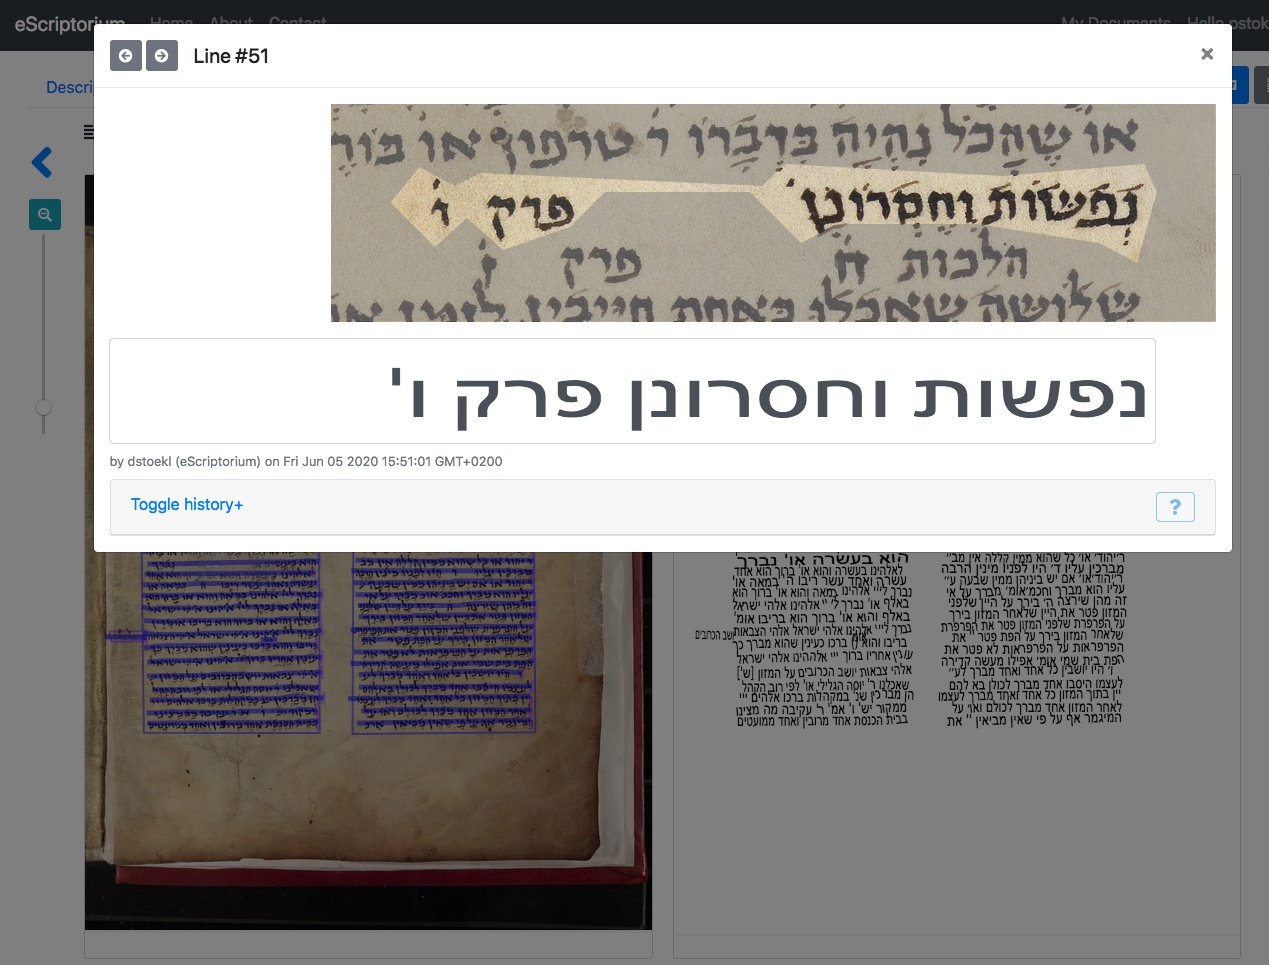
\includegraphics[width=0.9\textwidth]{fig1.jpg}
	\caption{Entering and correcting lines of text in eScriptorium.}
	\label{fig:fig1}
\end{figure}

\begin{figure}[h]
	\centering
	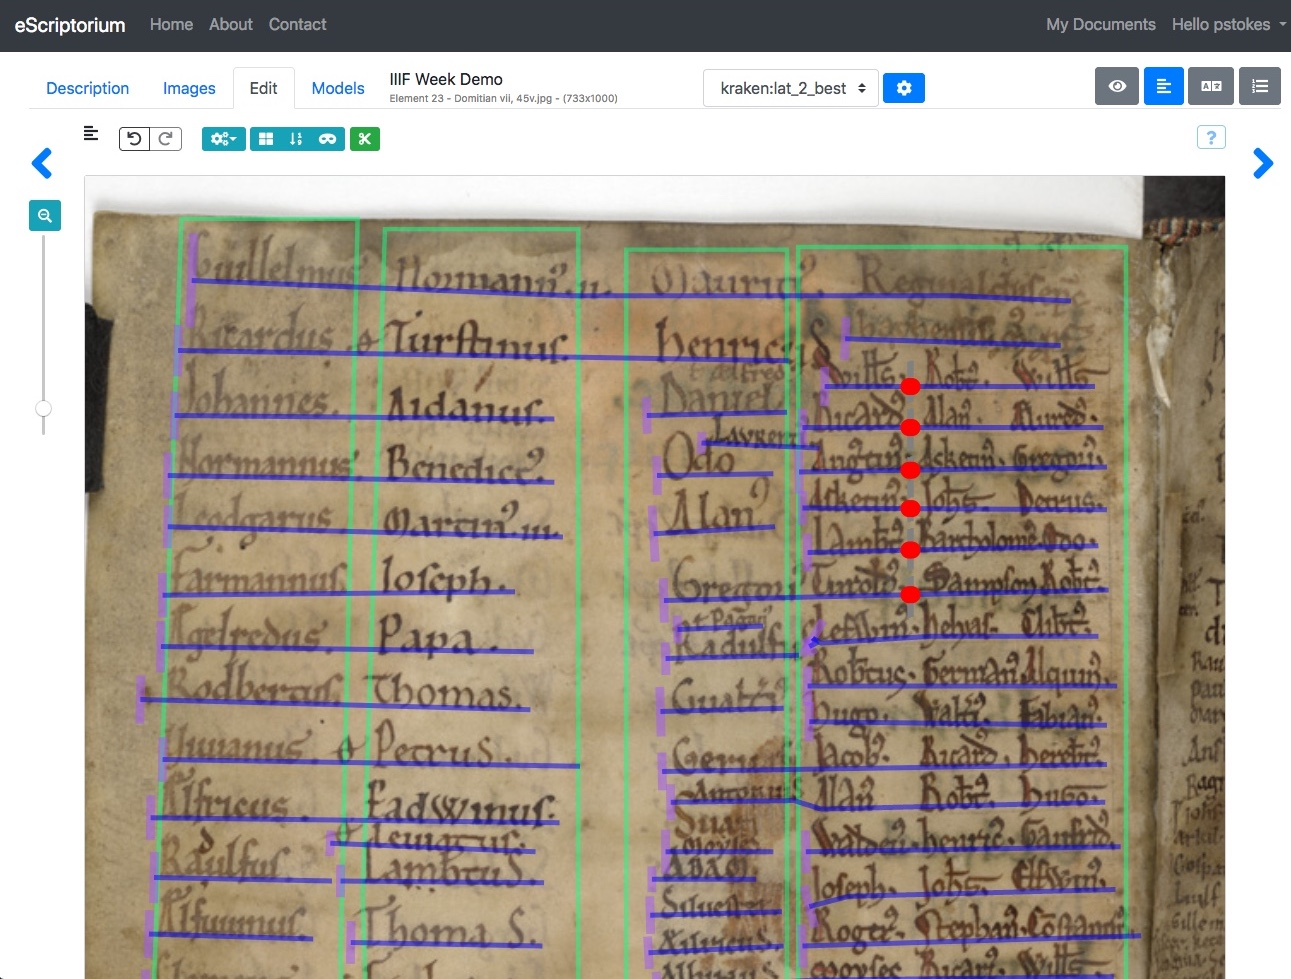
\includegraphics[width=0.9\textwidth]{fig2.jpg}
	\caption{Correcting automatic segmentation in eScriptorium. The
	manuscript image used in this screen-shot is a detail from London,
	British Library, Cotton MS Domitian A.vii, 45v. }
	\label{fig:fig2}
\end{figure}

In practice, these two steps for machine learning often comprise several
sub-steps. For instance, one may begin by preparing a certain number of pages
by hand, most often by typing them out manually (Figure~\ref{fig:fig2} and
\cite[n. 4]{stokes2020videos}). It may then be helpful to train the machine
based on this relatively small sample and then automatically transcribe some
more pages: the results may have numerous errors, but correcting these errors
may be faster than typing out the whole page. After manual correction, the
machine can be re-trained with this additional material, and then the
subsequent pages will have fewer errors and will therefore be faster to
correct. This process can then be repeated until the results are good enough to
be useful. How good is “good enough” depends very much on the use-case: it is
generally not possible to get perfect results, but it is often possible to get
over 99\% character accuracy, meaning correcting perhaps one or two errors per
page. Correcting this number of errors is very much faster than typing by hand,
and the correction may well be unnecessary anyway, since 99\% character
accuracy is more than enough for many purposes of distant reading and other
large-scale analyses, such as automatically identifying uncatalogued texts, for
most forms of NLP and NER, and so on. There are also ways of speeding up this
process, for instance by taking an existing transcription of the same text
elsewhere, importing it into eScriptorium, and then adjusting it to match this
particular exemplar, or taking examples of other transcribed texts that were
written in scripts very similar to the new text, and training on those.

\section{State of the Art in Current OCR/HTR}

For the more technically-minded readers, it is helpful at this point to
understand the current state of the art in systems for manuscript OCR/HTR.
Feature-complete systems at the time of writing include Kraken but also
Tesseract 4 and Transkribus. Broadly speaking, these systems work in similar
ways for automatic transcription, and they give similar results in terms of
accuracy, but they differ significantly in areas such as their ability to cope
with complex “non-standard” page layout or “unusual” script (as seen from a
modern Western point of view), and the degree of openness in terms of Open
Source software but also in the ability to import and export data and trained
models, points which are discussed in the following section.

These current systems are generally line-wise text recognizers: that is, text
images are transcribed a whole line at a time in contrast to the
character-by-character approach which is employed in traditional OCR for
printed text (such as in Tesseract 3 and Sakhr). The line-wise transcription is
usually performed by a recurrent or hybrid convolutional neural network which
has been trained specifically for a particular script or even a specific hand,
depending on the complexity and variability of the writing. All modern systems
are trained with an implicit alignment between the desired textual output and
the input images, most often through what is known as the CTC loss function\cite{graves2006connectionist}.
The primary benefit of this alignment is easier acquisition of data for
training, as the laborious labelling of single characters is replaced with the
much simpler transcription of whole lines. 

Before transcribing the text, a modern system needs first to identify the lines
on the page, and this is handled by a layout analysis (LA) module, the exact
functionality of which depends on the nature of the text transcription module.
Character classifiers require the extraction of single glyphs from the page by
the LA system, a process which can be difficult for cursive scripts, while
line-based systems can use whole line extraction techniques which are more
versatile and script-independent. The major technical difference between
different HTR packages lies in this LA module: how it models lines and if it
can be adapted to new kinds of documents. Tesseract and Ocropus retain
hand-crafted, non-adaptable computer vision methods that output rectangular
boxes around the lines. These work reasonably well for printed documents and
clean handwriting but cannot reliably process complex manuscripts, especially
if the lines of text are curved or otherwise do not fit naturally into these
boxes. Recently, new forms of LA use the baselines of the text instead of
boxes, and this has been successful in dealing with highly complex material
containing slanted, curved, and rotated lines\cite{diem2017cbad}. Methods following this
paradigm are popular in the research community but actual implementations are
currently limited to Transkribus and Kraken/eScriptorium. 

In addition, a wide variety of research algorithms can also be found in the
literature but which have not yet been implemented in OCR systems. These
include systems that merge the steps for layout analysis and transcription
\cite{wigington2018start}, or methods that are optimized to extract text from
noisy environments such as natural scenes\cite{wang2011end}.
 Another active field of research in computer science is in
methods to decrease the manual labor required to successfully train machine
learning algorithms through approaches such as domain adaptation (transforming
models trained on one kind of document to another), semi-supervised learning
(training on partially labelled examples), and wholly synthetic manuscript
pages (training the machine on “artificial” images so that it can learn to read
the real ones)\footnote{One recent example among others is
\cite{kang2020ganwriting}} Nevertheless, it remains that the creation of these
example cases or “ground truth” for the computer is the longest and most
laborious part of the process for the end user, and it may even seem
contradictory that one
must manually transcribe many pages in order for the computer to transcribe
automatically. Indeed, if one only has a very small corpus, or if the range of
different scribal hands or styles of writing in that corpus is large, then it
may not be worth the effort to use these automatic methods. However, if the
corpus is large and homogeneous enough that the computer can train to a
sufficiently high level for your needs, then, once this initial groundwork is
done, the results afterwards can be spectacular, with thousands or even
millions of words being transcribed automatically at literally the click of a
button. Nevertheless, it should not be surprising that there is no “magic
solution” that can instantly solve all cases. As we know very well, texts are
extremely complex objects, with a great deal of variety in terms of layout,
format, structure, style of script, and so on, and it takes us human beings
many years of specialized training to learn to read them. This complexity makes
them interesting and worthy of years of study, but it should come as no
surprise that it also makes them difficult to treat with a machine. 

\section{Openness and Import/Export of Images, Texts and Models}

In addition to the flexibility and adaptability to different writing systems,
another of the core principles of both Kraken and eScriptorium is that of
openness. The software for both Kraken and eScriptorium is open-source and free
for anyone to download, use, and modify. More significantly, though, the
framework is designed to allow for the easy import and export of images,
transcriptions and trained models, and this is particularly important for a
number of reasons. As we now know very well from experience, a closed system is
extremely risky in terms of sustainability, since if you are locked into a
given system then you become entirely dependent on it: if it ceases to function
then your project is potentially in jeopardy, and one can easily become hostage
to any future developments, such as if a free service becomes paid-for. It is
therefore always of the utmost importance that one uses standards-compliant
data, and that this data can be freely imported into and exported from
different pieces of software, in order to avoid dependance on any one piece and
thereby help ensure the longevity of the process as a whole. Equally if not
more important in the case of OCR/HTR is the ability to import and export
trained models in particular which is important on both scholarly and practical
terms. From a scholarly point of view, there are very real questions around
scholarly transparency and accountability in the use of machine learning. If we
are preparing transcriptions automatically in this way then naturally the
results will be influenced according to the training data that we have provided
to the machine. As discussed above, there are different standards and practices
for transcription, and the types of document and script that are used in the
ground truth will inevitably influence the results. Other scholars will
therefore need access to the ground truth and trained models in order to
understand exactly how the text was obtained, to evaluate if it was appropriate
or not, and to anticipate potential biases and errors.\footnote{A simple
example of an error resulting from this point was a project which attempted to
automatically identify authorship in vernacular Old English texts, but without
controlling for different editorial practices in the sources: as a result, the
project was successful in identifying editors but not authors. See further
\cite[pg. 54-56]{stokes2009digital}} From a practical point of view, the
process of compiling ground truth is often laborious as we have seen, and in
fact on a commercial level, very large-scale datasets of high-quality ground
truth are extremely valuable, which is part of the reason why multi-billion
dollar corporations are so keen to access our e-mails, labelled photographs,
and so on. In addition, the process of training a model is also relatively slow
and intensive. This is of less concern to the average user in the Humanities,
since we can simply leave the computer to “do its thing” while we get on with
something else. Nevertheless, training Deep Learning systems like Kraken is
very intensive for the machine, and it can take weeks on a normal home
computer. The process is very much faster if one has access to a High
Performance Computing (HPC) center with specialized hardware, but very few
scholars in the Humanities have this access, and in any case the process uses a
relatively high amount of electricity with financial and
ecological implications.\footnote{As just one example, the GPU units that the
eScriptorium team are currently putting in place will have an estimated running
cost of approximately €10,000 per year.} Fortunately, the training is the
intensive and slow part, and once this is done then the model can be used
relatively quickly and easily for the segmentation and transcription. However,
this again illustrates the benefits of exporting and sharing models. If I can
train my model in an HPC center, and then download it and send it to you, or -
even better - publish it on an open repository, then you and anyone else can
take my model, upload it to your instance of eScriptorium (or Kraken, or some
other
system), and use it from there. You may need to retrain it to fit your specific
documents, but as long as our documents are sufficiently close then the
training that you need to do can be significantly reduced both in terms of time
and the amount of ground truth. You would then ideally also publish your
re-trained model in a public repository, and in this way we can build up a
shared collection of trained models, thereby reducing significantly the
computing time and energy that is currently being wasted on the redundant
training of many different models on what is essentially the same script. More
specifically, Kraken and eScriptorium both allow users to export and import
models, for instance downloading them to their personal computers to do with as
they wish. Kraken is also directly linked to Zenodo, which is a large-scale
public international repository for research data. This means that one can
decide at any point to publish a model to Zenodo, and the system will then take
care of the publishing meaning that the model will be saved for the long term
according to best practices in data archiving including the automatic
assignment of a persistent identifier (a DOI) for future reference. Managing
this successfully requires significant care in documentation and metadata, as
future users of an existing model will need to know which standards of
transcription were used, along with which sample images and so on, and this in
turn requires that the entire ground truth also be published along with the
model.\footnote{For further discussion of this and other related problems, see
(for example) OCR-D \cite{ocrdtrans}.}

\section{Some Challenges for a Multi-Script VRE}

The discussion so far presents eScriptorium as it stands at the time of
writing. Although very much still in development, it is already being used by
numerous teams in several different instances across Europe and the United
States.\footnote{As well as Scripta and RESILIENCE, other example projects
include OpenITI AOCP (\url{https://www.openiti.org}), LectAuRep, Sofer Mahir
(\url{https://sofermahir.hypotheses.org}), DIM STCN
(\url{http://www.dim-humanites-numeriques.fr}), and CREMMA
(\url{https://www.dim-map.fr/projets-soutenus/cremma/}), among others.} There
are, however, numerous challenges that remain if the project is to achieve its
goals. Aside from technical details of implementation, it
seems at this point that the most significant challenges lie in the goal of
being as close as possible to working with any script. Indeed, it is already
clear that this is not truly possible: for instance, as mentioned above, the
automatic transcription module of Kraken applies a line-by-line approach, but
this assumes that the text is in fact written in lines (or that it can be
approximated as such), an assumption that does not hold for hieroglyphic
scripts like Mayan or ancient Egyptian. Indeed, the question of text direction
is more complex than one might first imagine. On the face of it, the situation
is simple enough: most scripts read in lines from left to right and then top to
bottom (such as Greek and Latin), or in lines from right to left and then top
to bottom (such as Hebrew or Arabic), or in columns from top to bottom and then
left to right (as is often the case for Chinese and Japanese). There are,
however, other cases, such as lines read from top to bottom and then right to
left (such as Mongolian), or columns read from bottom to top (such as some
inscriptions in Old Javanese). Furthermore, some scripts like Latin are
(usually) written on a baseline, while others like Hebrew are (usually) written
from a top-line, and Arabic can be written along short diagonal segments which
form a line overall. Writing can also be circular, for instance on coins, or
spiral-shaped, for instance on prayer-bowls, or radiating out from a central
point, for instance in Arabic marginal glosses (Figure~\ref{fig:fig3}), or in very complex
shapes that form pictures, for instance in micrography or calligrammes. The
situation is even more complex in multigraphic contexts, that is, where
different writing-systems are mixed in a single document, such as
seventeenth-century liturgical manuscript written in Chinese and Hebrew, to
take just one example from many thousands\footnote{Hebrew Union College MS 926,
available at \url{https://mss.huc.edu/manuscripts/ms-926/}}. The international
Unicode standard for representing the world’s writing systems in computers
describes an algorithm for treating bidirectional documents (such as mixing
English and Arabic); this standard is in its forty-second revision at the time
of writing and currently extends to nearly eighteen thousand words, or around
forty-five pages if printed. This illustrates the complexity of simply
displaying a typed document with different directions of script, let alone that
of automatically transcribing such a document from an image and then presenting
it in an interface where the user can correct the lines, regions and
transcription, with all the text being displayed in the correct directions as
required.

\begin{figure}[h]
	\centering
	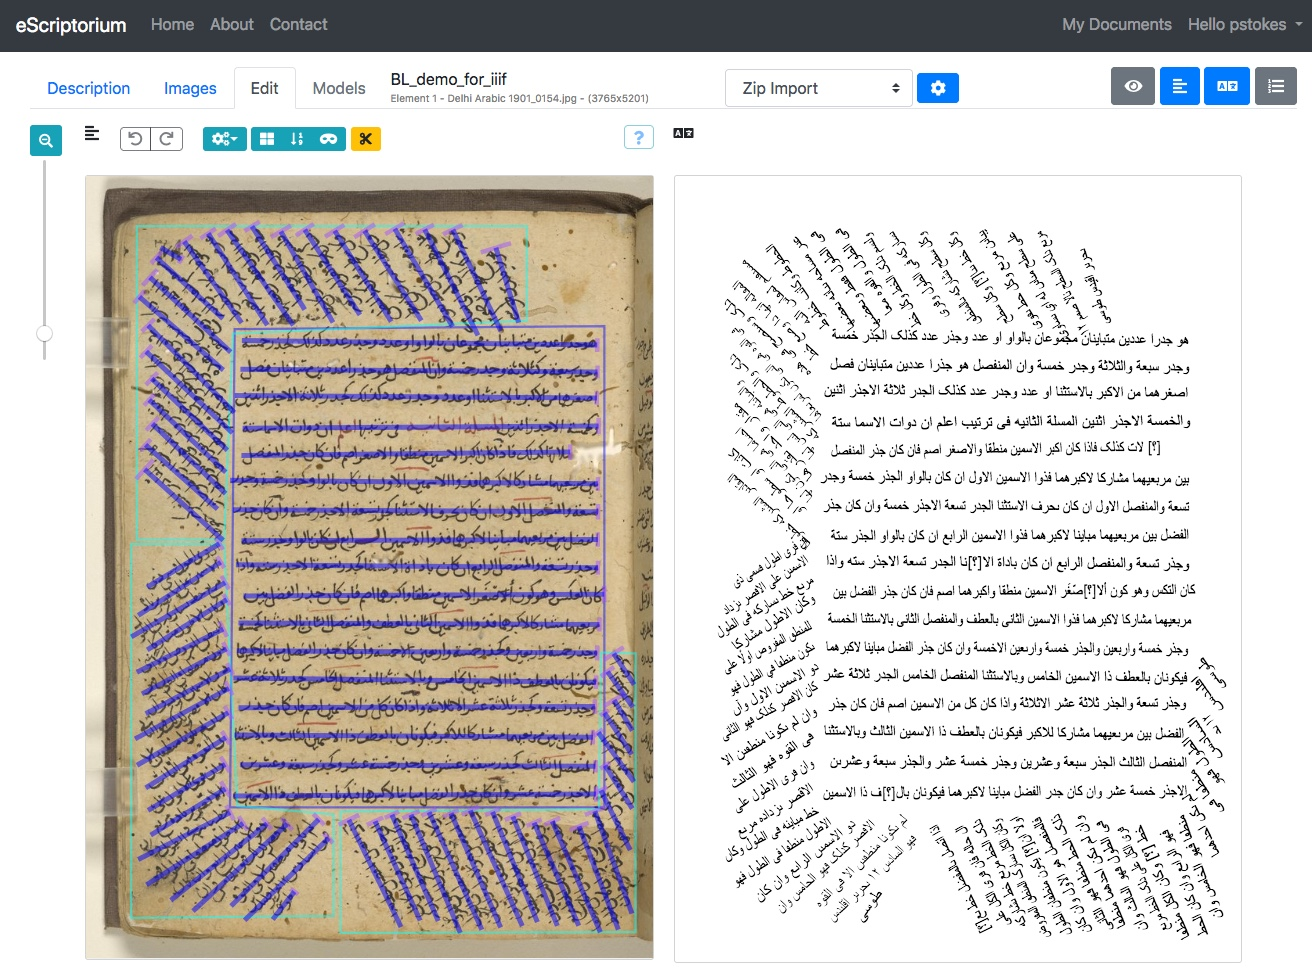
\includegraphics[width=0.9\textwidth]{fig3.jpg}
	\caption[Visualizing complex page layouts in eScriptorium]{Visualizing complex page layouts in eScriptorium. The
	manuscript image used in this screen-shot is out of copyright and is
	from British Library and \protect\cite{rasm2019res}.}
	\label{fig:fig3}
\end{figure}

This variety of writing-systems, and particularly the need to cater for so
called “rare” and historical scripts, introduces further challenges than
directionality. By definition, “rare” languages and scripts do not have large
corpora and are not already well catered for by existing software and methods.
Indeed, the very nature of Deep Learning is that, as we have already seen, it
requires large amounts of pre-existing material, and in general the more such
material the better (provided that the data is sufficiently representative).
This means that, almost by definition, methods that rely on “big data” are not
appropriate for “rare” languages and scripts. In practice these methods can
usually be used anyway, to some extent, as long as the corpus is not very small
or very heterogeneous, but they will almost always be small “boutique” projects
that will not have the support of large companies, for both better and worse,
or reusability across domains. Furthermore, some of the basic techniques for
improving the results of OCR/HTR will not work in these cases. For instance, it
is very common to use some sort of statistical language processing to correct
errors in the OCR of modern texts: a very simple example is to run a
spell-checker on the result, but more complex examples attempt to automatically
analyze the language and attempt to correct errors based on what is or is not
linguistically possible. Such an approach can improve the transcription
considerably, but it requires a pre-existing model of the language, so that the
computer can recognize what is and is not likely to be an error. However,
searches for a spell-checker for (say) Old Vietnamese is very unlikely to bear
fruit any time soon, if ever, and indeed the same holds for accurate
statistical models of orthographically varied historical writing in general.

\section{Different Points of View}

There is, however, a further aspect of this: as those of us in the Humanities
know very well, there are many different conventions and possibilities when
preparing editions. Despite the claims of some that a transcription must be a
simple reproduction of “what is on the page”, it is nevertheless clear that a
written text contains an effectively infinite amount of information, and any
transcription is necessarily an active selection and, in a sense, translation
from one system of writing to another.\footnote{Discussions of this include
\cite[pg. 464-472]{pierazzo2011rationale}, \cite[pg.
85-101]{pierazzo2016digital},
\cite{huitfeldt2008transcription,sperberg2018interpreting}, and \cite[pg.
20-29]{robinson1993guidelines}.} Even Latin texts have different conventions
for transcription, depending on whether the context is Classical or Medieval,
whether paleographical,  epigraphical or papyrological, and so on, and the
complexity multiplies enormously when considering practices for languages such
as those of South-East Asia or even the Ancient Near East.\footnote{One example
of a transcription guide for such languages is \cite{balogh:halshs-02272407}}
It is therefore impossible and indeed undesirable that the computer
automatically produce a transcription without any guidance from the user, since
it is impossible to know a priori which standards of transcription the computer
should follow. One can certainly imagine pre-preparing a list of common cases,
following conventions established by significant scholarly bodies, and this
would indeed be very useful and desirable, but it still seems certain that many
other cases would remain. This need to accommodate different standards makes
the reuse of models more difficult, since it increases the degree to which
models must be retrained for specific cases. The challenge goes much further
than this, however, and extends to the basis of any VRE for manuscript studies
or textual editing, since it also means that any VRE which will be used by a
wide range of people must be able to accommodate these different standards.
Extending the workflow from transcription to edition introduces further
complexities, as there are (also) many different types of edition, and the
variety in editions is (probably) greater than that of transcriptions. Ideally,
a single VRE should accommodate all standards and types of edition, as well as
all standards of transcription, for all writing-systems written on all
supports. Such a flexibility is possible, but it comes at a cost: either the
interface must be extremely complex to account for all the different options,
or it requires some level of programming in order to produce a customized
interface which is specific to a given project. Indeed, this is perhaps the
biggest challenge faced by the challenge of the Text Encoding Initiative (TEI).
Many have complained that the TEI guidelines for text encoding are extremely
complex and unwieldy, and that they do not proscribe a single convention for
transcription meaning that, in effect, they are not a true standard. However,
if the TEI Guidelines did impose a single convention then they would
immediately become unusable for all those who want or indeed need to use other
conventions. Texts are different, and editions and research projects have
different goals and therefore different needs, even those projects that are
studying the same texts.\footnote{An example of this is described by
\cite{stokes2010project}}  In practice, then, the TEI is a sort of
“meta-standard”, from which one can then specify more restricted and
proscriptive standards for particular contexts, with one of the more successful
examples being Epidoc for editions of inscriptions.\cite{epidoc} VREs and other
tools for the preparation and publication of digital editions face a similar
challenge: it is certainly within the bounds of technology to develop a simple
process whereby one can produce a transcript or even publish an edition very
easily in a relatively small number of clicks, but this necessarily means that
most of the decisions will be taken from the researcher and put into the hands
of the tool-developers. Conversely, processes can also be developed which give
manuscript specialists control over fine details according to their own needs,
but this means complex interfaces and/or the need to actively write code at
some level to customize the process.

This need for different standards, methods and points of view extends well
beyond transcription and editions, and indeed goes to all forms of manuscript
studies and indeed to all scholarly research in the humanities.  Armando
Petrucci and Collette Sirat have both made similar observations for
palaeography\footnote{Some concrete examples of the impact of transcription on
interpretation are given by \cite[pg. 50-54]{stokes2020b}}:

\begin{displayquote}[{\cite[pg. 70-71]{petrucci2001descrizione}\footnote{“In fact, every palaeographical terminology is connected to a particular historical vision of the phenomenon of handwriting ... but all terminologies prove legitimately useful nonetheless, if they are founded on valid methodological premises and rigorous graphical analyses” (our translation).}}]
Infatti ogni terminologia paleografica è legata ad una particolare visione
storica del fenomeno scrittorio \dots ma legittimamente utilizzabili risulteranno
comunque tutte quelle fondate su premesse metodo\-logiche valide e su rigorose
analisi grafiche.
\end{displayquote}
\begin{displayquote}[{\cite[pg. 310]{alma991005247569705596}}]
Two things which are similar are always similar in certain respects. \dots
Generally, similarity, and with it repetition, always presupposes the adoption
of a point of view: some similarities or repetitions will strike us if we are
interested in one problem or another.
\end{displayquote}

This may seem obvious, but in fact it raises a fundamental epistemological
question: annotation and comparison are core tasks of scholarship, and have
been identified as two of the six “scholarly primitives” which underly all of
our work.\footnote{These “scholarly primitives” are from an influential talk by \cite{unsworth2000scholarly}.} However, annotation, or description, depend on terminology, as
indeed does discovery, another of Unsworth’s primitives, but as Petrucci has
noted, there is no single terminology which can be claimed as “the” valid one
over all others. Similarly, Sirat and Popper have noted that comparison also
requires a point of view, and different problems require different comparisons
and therefore different points of view. This poses a very significant challenge
to VREs, and indeed to the ideal of interoperability and related areas such as
Linked Open Data. In addition, the fundamental principles of machine learning
itself, as a mere kind of statistical inference, can cast doubt on the
scholarly value of the automatic productions of these methods when “hidden”
inside VREs, with their design assumptions and limitations remaining relatively
opaque to the humanities users even in open systems. In principle, different
terminologies can be related through ontologies and other tools, such that one
can record for both human and computer use that two given terms are close in
meaning, exact matches, related, broader or narrower in scope, and so on, and
in this way one can link different terminologies, at least in
principle.\footnote{One important example of such a schema is the Simple
Knowledge Organisation System (SKOS), for which see \cite{miles2009skos},
esp. §10 Mapping Properties.}
However, this is a complex and laborious process, and it also requires a very
deep understanding of both terminologies as the scope for misunderstanding and
error is enormous. We must therefore consider how to design VREs to enable
different points of view, which includes allowing for different terminologies,
different interfaces, different ways of presenting, annotating, comparing,
searching and otherwise working with the data. Indeed, as Elena Pierazzo has
observed, the text itself is only one part of the scholarly work and
interpretation in an edition, and Johanna Drucker and others have shown that
the interface generally is interpretative and embeds specific methods and
viewpoints, and it therefore necessarily excludes
others\cite{pierazzo2011rationale,drucker2014graphesis}.  For this reason, it
seems unlikely that there can ever be a single VRE or other system which
responds to all requirements, but instead perhaps we must accept that there
will always be many different tools and frameworks. Certainly we must follow
existing standards where these are available: otherwise there is no hope for
interchange or data sharing, and our material is certain to be lost very
quickly once our custom tool is no longer maintained and our custom data is
therefore unreadable. Similarly, the best option remains to follow standards
and to use tools that allow for the ready import and export of data, including
trained models in the case of machine learning. In this way we have some chance
of moving between different tools, frameworks and VREs as necessary, taking
advantage of those that best respond to the point of view that we need for a
given problem at a given moment. This also suggests favouring smaller modules
that can be pieced together into different workflows as required, rather than
large, centralised, monolithic VREs, and the piecing together in turn requires
at least some understanding of data and (probably) basic programming. This
should not be of concern to Classicists or others in the Humanities: certainly
software development is a highly skilled profession that requires specialised
training, but the basics of Python and XSLT are very much easier to learn than
the complexities of Greek or Latin.
